\chapter{绪论}

\section{研究背景}

近年来,工业机器人凭借着其极高的效率和进度,不断取代人力加速生产,在例如3C制造业,五金加工,家具生产等各种离散制造行业取得了卓越的成绩。这些离散制造业普遍具有短周期,多种类,小产量等柔性制造特性,产品迭代频率非常高,生产节奏也非常快。这就给工业机器人快速部署,灵活调整提出了非常高的要求,而传统工业机器人的编程模式对这种要求较难满足。因此,如何提高工业机器人的易用性(Ease of Use),特别是简化装配作业编程(Ease of Programming),已经成为工业机器人自动化领域亟需解决的一个问题。演示编程(Programming by Demonstration, 简称PbD)是目前一个非常前沿的工业研究课题,通过由机器人系统从人的操作演示中理解并提取关键信息,进而将该信息自动编程为机器人可执行程序以及模型参数,从而使机器人完成相应的操作\cite{billard2008robot}。该方法能够提供一种新的向机器人传递信息的方式,是简化机器人编程的重要途径\cite{argall2009survey}。

% 对零件或者通用物体的位姿估计是众多演示编程示教任务中的一个基本核心任务。
演示编程技术中有一个关键环节在于对工业机器人的工作点位进行指定,其中包括机械臂对某个工业零件进行抓取或放置。目前演示编程技术应用过程中,更多采用的方式是通过事先设置较为固定的零件位置,使得机械臂在工作期间只要按照既定的程序进行工作便可。但由于工业机器人的操作点位的数值空间和人的直观空间感受存在较大的差异,人为设置固定的零件数值位姿成为一件非常繁琐复杂的事情,给工业机器人的部署带来了极大的不便。因此,利用物体的位姿估计算法直接给出物体的位姿,进而反算给出机械臂应有的工作点位,可以极大程度上解决这一问题。除此之外,在很多实际生产流水线上需要对零件进行分拣,将零件从杂乱的分布整理为整齐规则的顺序,这时候就可以利用物体位姿估计算法实现该过程的自动化,解放人力。

例如图1-1中工业环节所示,需要将一些零件从传送带或者Tray盘上抓去抓取进行装配,或者放置到下一个工业环节中去,这其中就须要工业机器人知晓零件的位姿。通常传统方法是通过将零件整齐有规律地放置在一些有卡位结构的传送带或者Tray盘中,使得零件相对于工业机器人的位姿是绝对固定的。用这样的方法的确能直接解决问题,但同时也带来了例如机械臂标定,Tray盘传送带标定等一系列附加问题。并且这些标定问题通常是非常繁琐,非常浪费人力物力的。再加上目前由于工业场景是多变和复杂的,特别是柔性制造领域,工业零件也随着需求的变化而日新月异,一旦零件规格发生变化或是工艺发生了更新,所有的生产就会立马收到限制,极大降低了工业生产效率。但如果有一套高效便捷的零件位姿估计系统,就完全可以解决上述所有问题,大大降低生产空档时间,提升产出效率。因此对零件的位姿估计的研究具有非常高的工业应用价值和学术研究价值。因此本文将针对零件位姿估计展开研究。

\begin{figure}[htb]
	\subfigure[工业机器人抓取Tray盘上的零件]{ 
		\begin{minipage}[b]{0.5\textwidth} 
		\centering
		% \label{fig:SubFigure1} %% label for second subfigure 
		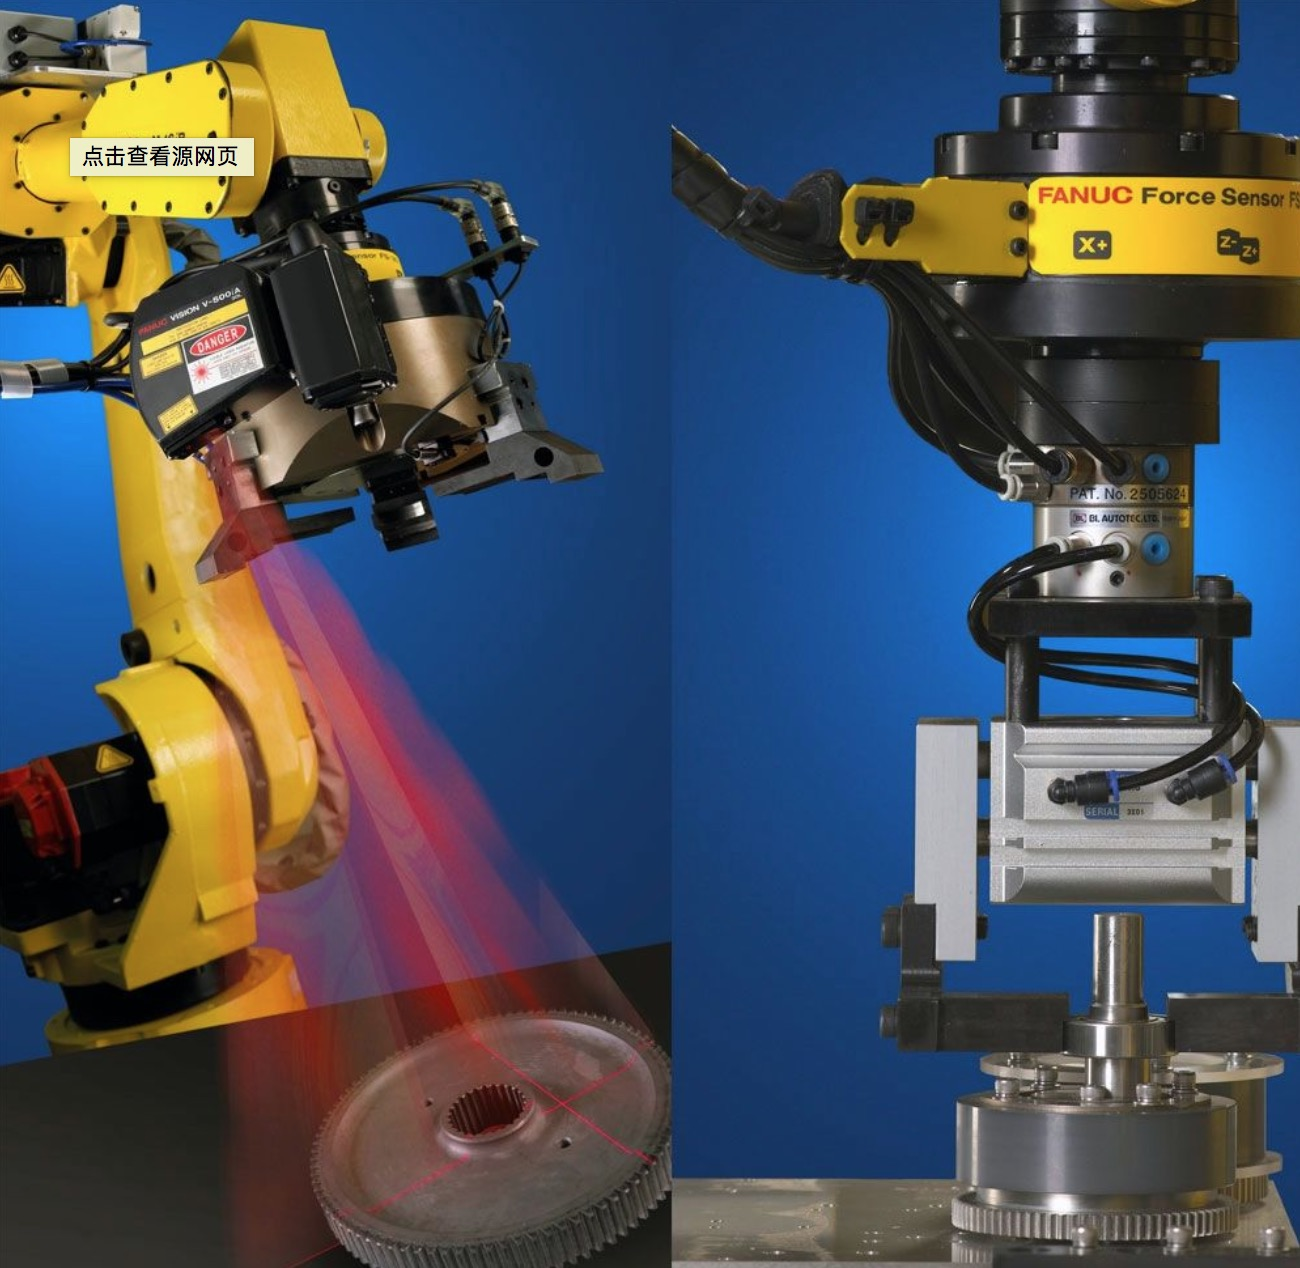
\includegraphics[scale=2.0]{./mypic/工业机器人2.jpg} 
		\end{minipage}}
	\subfigure[工业机器人抓取传送带上的零件]{ 
		\begin{minipage}[b]{0.5\textwidth} 
		\centering
		% \label{fig:SubFigure1} %% label for second subfigure 
		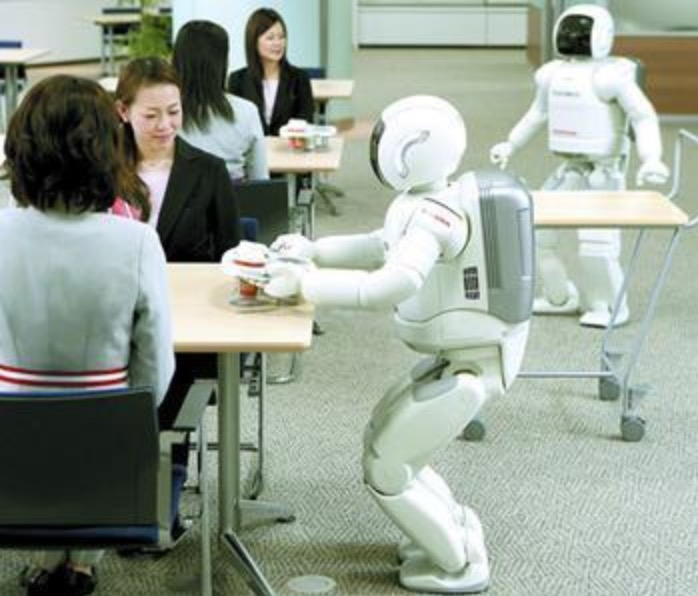
\includegraphics[scale=1.0]{./mypic/工业机器人1.jpg} 
		\end{minipage}}
	\caption{一些工业装配现场}
\end{figure}

在几乎所有工业环境中,计算机视觉是可以作为反馈的一种方便部署并且高效的方法。因此,计算机视觉已经成为了工业机器人研究领域中非常重要的一点。基于工业摄像头的计算机视觉是非常经典的研究内容,因为工业摄像头提供的高清RGB图像信息可以提供非常充足的环境信息,并且有很好的实时性。而近年来,伴随着例如Kinect,Leap Motion,RealSense等各种各样的面阵3D深度传感器的诞生,计算机视觉有了一个全新的维度。因此,针对这些3D深度传感器的计算机视觉研究掀起了一股热潮。

但由于目前物体位姿估计研究领域尚未给出一个较为理想的解决方案。特别在于位姿估计解决方案的易用性以及效率上,现有的算法均存在局限性大,计算效率低下无法实时计算等问题。本文将在此背景下,面向工业装配演示编程中对物体位姿估计的需求,利用深度相机这一新型传感器展开研究和开发,以推动演示编程技术以及工业机器人的自动化发展。


\section{研究现状与趋势} 

\subsection{物体位姿估计方法分类} % 随机森林与随机蕨 包括特征提取


物体位姿估计是一个非常大的领域。从目标角度来划分可以有人体姿势位姿估计、人脸特征点定位(五官位姿估计)、人脸朝向位姿估计、车牌位姿估计等各种其它实物的位姿估计。其中每一块内容都有非常多的研究人员投入,并且一直以来都有各种各样的方法和理论被提出,同时各个不同目标的位姿估计方法不断交融与碰撞产生更新颖更优秀的方法,持续促进着整个位姿估计领域整体的发展。但总体而言,物体位姿估计领域的各种优秀的方法可以被大致分为两种类型,一种是基于模版匹配的方法,另一种是基于模型回归的方法。两种方法各有优势也各有短处。

基于模版匹配的方法大致算法流程如图1-2所示。首先算法需要事先准备或者事先计算好大量的模版,这些模版中每一个都代表被测物体的一个位姿状态。为了节省计算机资源和存储资源,这些模版在实际应用过程中将通过特征的形式进行存储,作为特征描述库。特征描述随算法不同而各不一样,常见的一些特征描述有SIFT\cite{lowe1999object},SURF\cite{bay2006surf},BRIEF\cite{calonder2010brief},ORB\cite{rublee2011orb}等经典特征描述。这些特征描述往往具有较好的尺度不变性以及对不同光照影响下的稳定性。存储好这些带有位姿信息等模版特征描述之后,便可以在实际位姿估计过程中通过比对输入的新图像的特征描述与特征描述库里的模版,得到一个最为接近的模版,从而最后得到对应的物体位姿。
\begin{figure}[htb]
	\centering 
	% 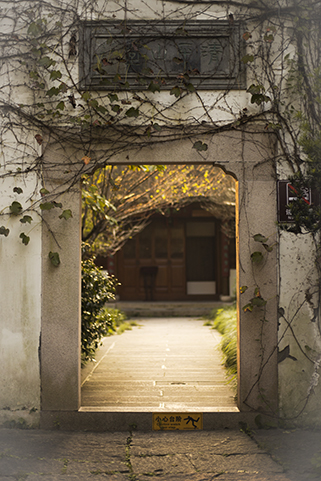
\includegraphics[width=\textwidth]{./Pictures/test.jpg} 
	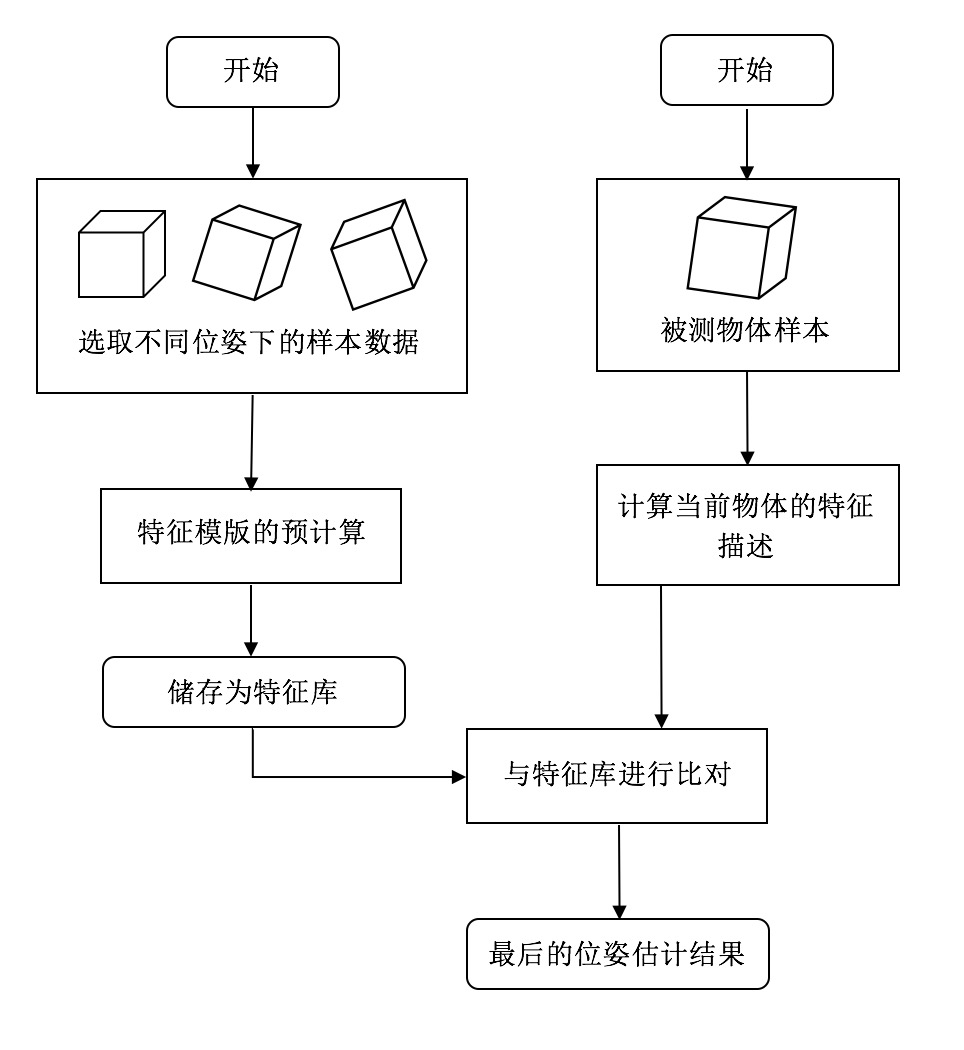
\includegraphics[width=0.8\textwidth]{./mypic/基于模版匹配的位姿估计算法流程图.jpg} 
	\caption{基于模版匹配的位姿估计算法流程图} 
\end{figure}

基于模型回归的位姿估计方法算法流程如图1-3所示。首先也是对目标物体进行特征提取,精准表达出物体的位姿特征。但是不同于基于模版匹配的算法框架,该方法在计算得到物体的特征描述之后不需要与实现准备好的模版库进行匹配,而是直接将位姿特征描述输入一个回归器里,通过回归器直接回归得到物体的位姿姿态。而其中这个位姿回归器则是通过事先大量的带真值标记的样本进行训练得到的。这其中的回归器可以是简单的线性回归,例如最小二乘回归等等,也可以是复杂的非线性回归例如SVM回归\cite{basak2007support}等。
\begin{figure}[htb]
	\centering 
	% 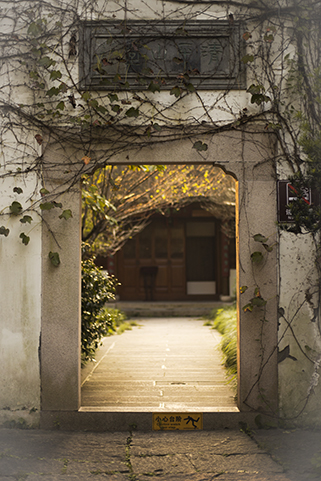
\includegraphics[width=\textwidth]{./Pictures/test.jpg} 
	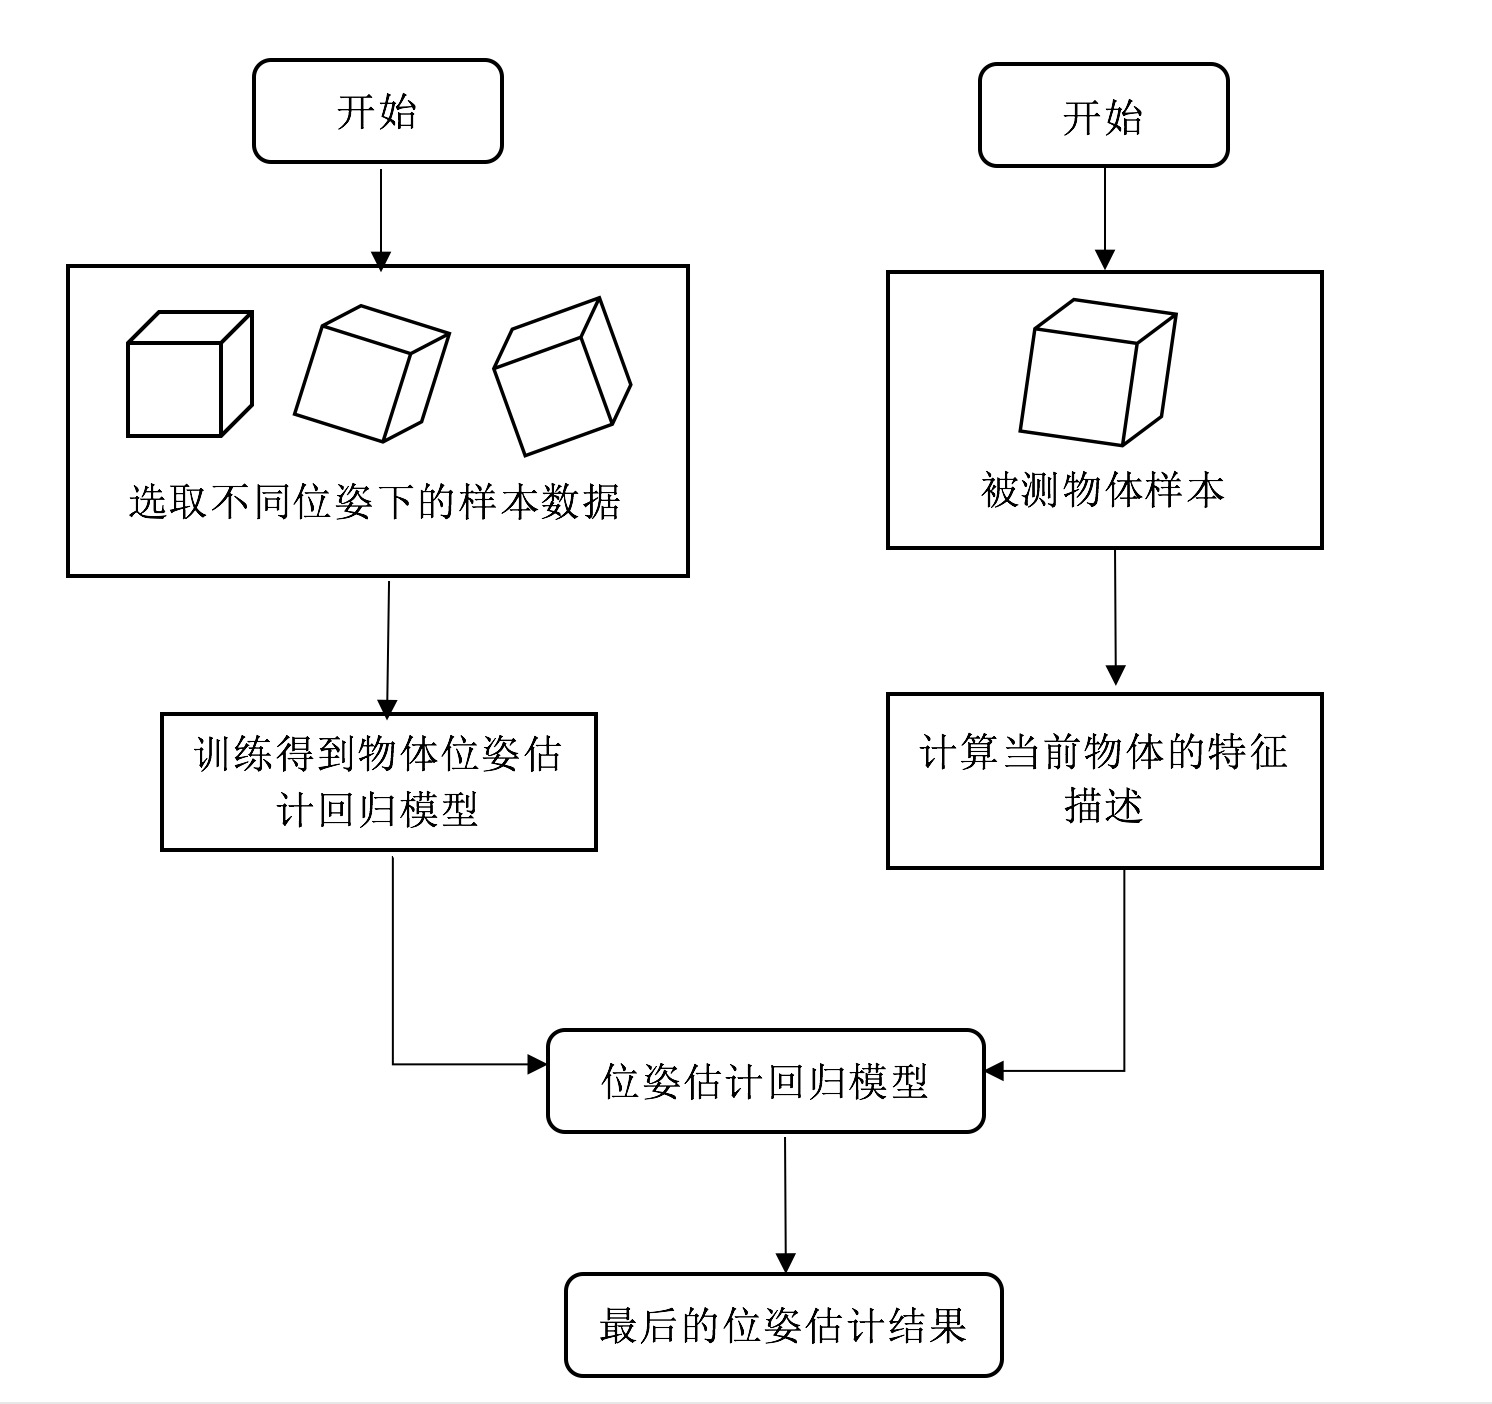
\includegraphics[width=0.8\textwidth]{./mypic/基于模型回归的位姿估计方法算法流程图.jpg} 
	\caption{基于模型回归的位姿估计方法算法流程图} 
\end{figure}

可以直观感受到,基于模版匹配的物体位姿估计方法通常需要较大的预存储空间,因为通常情况下一个物体的姿态会有非常大的变动空间,即使采用离散采样的方式来记录整个位姿空间下对应的各个位姿特征描述,也会有极大量的数据需要存储。一方面这样大量的存储会带来物理资源的需求,同时在进行位姿估计的过程中如果要匹配一对最接近的位姿特征描述,其计算量也是相当大的。相比之下基于模型回归的方法则有更为有竞争力。基于模型回归的方法虽然需要在事先通过学习大量的带标记的样本来得到物体的位姿回归器,但是位姿回归器在经过学习之后得到的模型通常只占有有非常小的数据存储空间。此外,当新的样本输入之后,位姿回归器根据其特征描述可以非常迅速地给出物体最终的位姿结果,不需要大量的计算资源。因此基于模型回归的位姿估计方法在实际应用过程中往往具有相对较强的竞争力。

在基于模型回归的位姿估计框架中,有很大一部分杰出的算法都用到了集成学习算法,并且考虑到位姿回归问题在回归空间上的高度复杂性,采用了非常新颖的级联回归算法进一步提高回归模型的回归能力。因此集成学习算法开始被大量关注并研究,同时级联回归算法框架也被不断应用到不同的领域当中。


\subsection{集成学习算法} % 随机森林与随机蕨 包括特征提取

集成学习方法通常指那些可以生成大量不同模型,并且可以将这些模型以一定的方式进行组合得到新的模型,从而用语解决分类或者回归问题\cite{mendes2012ensemble}。集成学习在很多情况下也被称为Committee、Classifier Fusion、Combination以及Aggregation等\cite{valentini2002ensembles}。从[\citenum{liu2000evolutionary}][\citenum{breiman2001random}][\citenum{rodriguez2006rotation}]等一些文章中可以看出,集成学习在近几年来取得了非常好的成绩,其优势具体表现在它相比单一的模型具有更加强大的鲁棒性以及准确性\cite{garcia2005cooperative}。其原理图如图1-4所示。

\begin{figure}[htb]
	\centering 
	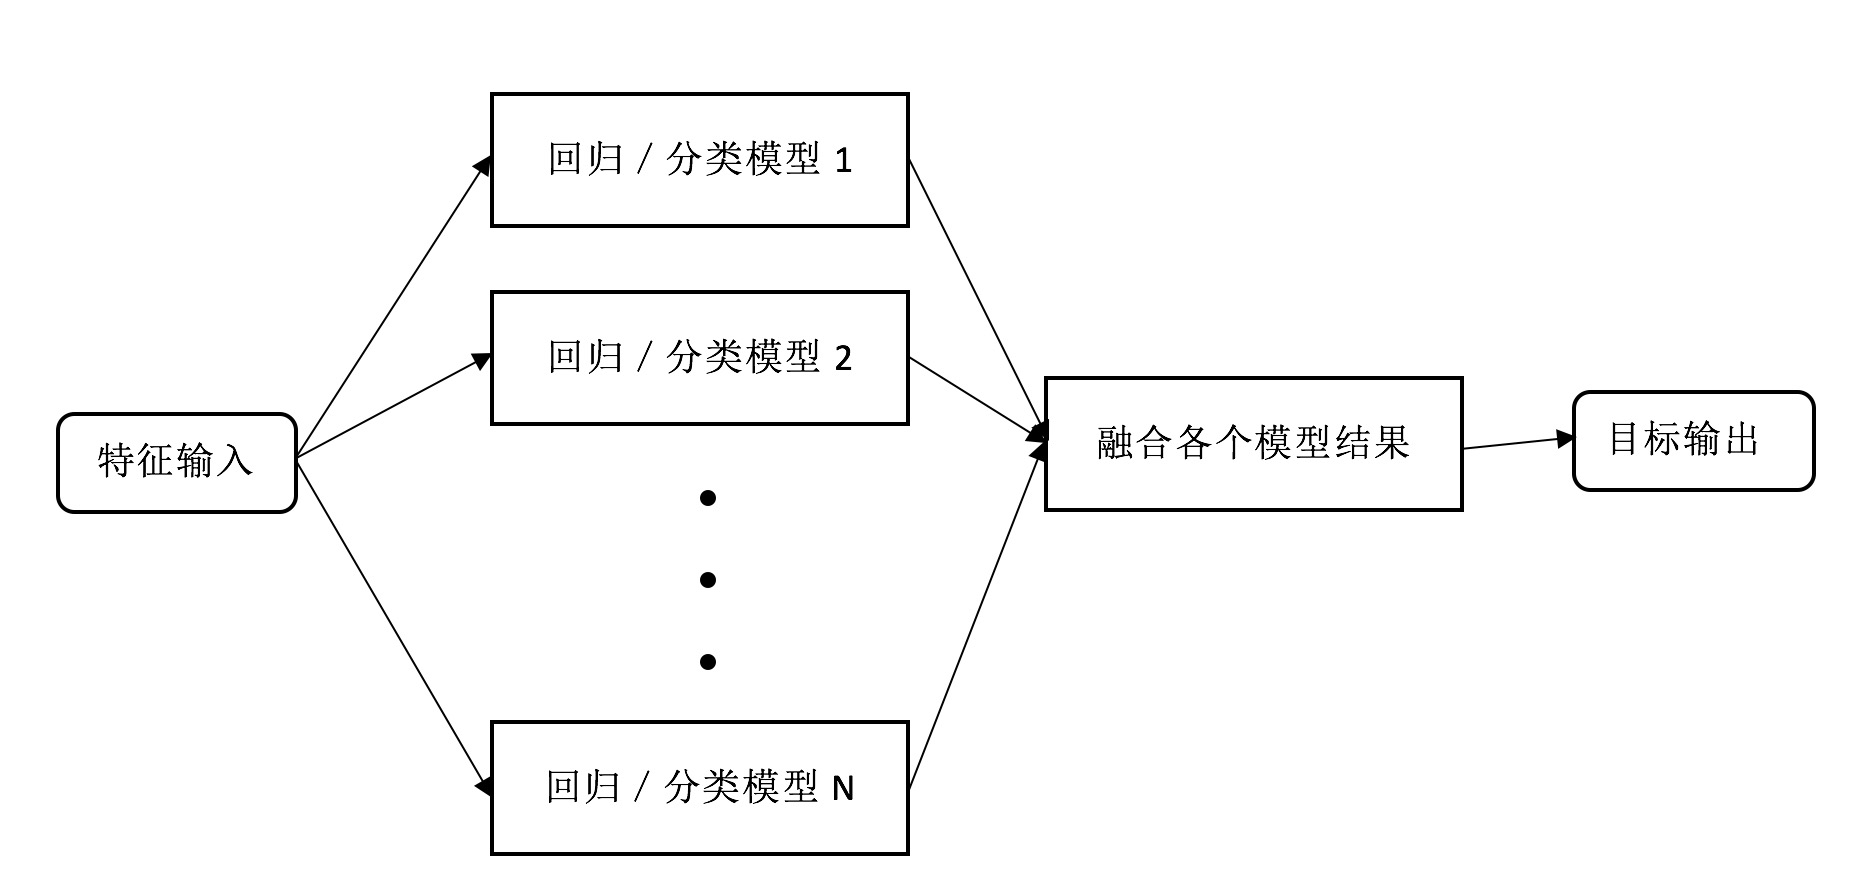
\includegraphics[width=0.9\textwidth]{./mypic/集成学习算法基本原理图.jpg} 
	% 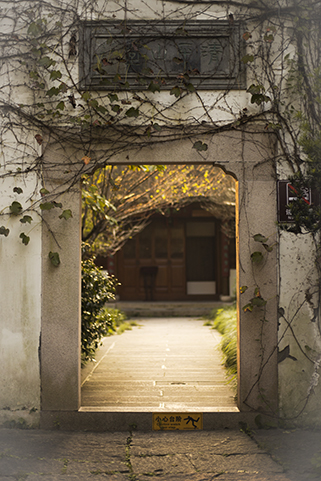
\includegraphics[scale=1.0]{./Pictures/test.jpg} 
	\caption{集成学习算法基本原理图} 
\end{figure}


集成学习方法通过将不同模型进行组合得到新模型,按照这些子模型的种类关系可以将集成学习方法大致分为两种,分别是异态集成学习和同态集成学习。

异态集成学习是通过将种类不同的分类器进行集成,其中最为主要常见的两个主要方法为Wolpert等人提出的叠加法(Stack Generalization)\cite{wolpert1992stacked}以及Vilalta等人提出的元学习法(Meta Learning)\cite{vilalta2002perspective}。叠加法的思想是通过将基本的模型分布在多个层次上,再通过这个多层模型完成学习任务。William W等人则利用这种思想构造处了一种更加新颖的串行学习算法,并指出这种串行算法相比不串行在性能上有较大提升\cite{cohen2005stacked}。元学习法的主要思想则是通过训练一个元模型来对所有的基本模型的输出进行进一步处理,最终得到问题输出结果。其主要包括两种方法:仲裁法(Arbiter)以及合并法(Combiner)。仲裁法是元模型从所有基本模型的输出结果中选择出合理的结果作为最后输出,例如投票方式。合并法则是通过用某种组合方法把所有基本模型的输出合并成最终输出,较为常见的Bagging\cite{breiman1996bagging}、Boosting\cite{schapire1990strength}等集成方法都是属于合并法。

同态集成学习方法则是指被集成的基本模型都应该属于同一种类的模型,仅仅只是这些基本模型之间的参数有所不同。同态集成学习模型主要有基于朴素贝叶斯的集成方法、基于决策树(Decision Tree,简称DT)的集成方法\cite{kearns1996boosting}、基于人工神经网络(Neuro-Network,简称NN)的集成方法\cite{zhou2002ensembling}\cite{zhou2002selectively}\cite{hansen1990neural}以及基于K—近邻的集成方法\cite{shen2007euk}等等。

异态集成学习方法由于需要提出众多不同模型才能构建更为强大的学习器,而通常情况下对于一个实际问题,要提出不同的模型来共同表述是一件非常困难的事情。相比之下,同态集成学习方法只需要提出一个简单的模型就可以完成复杂问题的学习。因此集成学习方法发展到现在,同态集成学习方法称为一种较为普遍并且表现优秀的一种学习方法,其中最为经典的一种同态集成学习方法就是随机森林\cite{breiman2001random}。随机森林算法是用随机的方式建立一个森林,森林里面有很多的决策树组成,随机森林的每一棵决策树之间是没有关联的。在得到森林之后,当有一个新的输入样本进入的时候,就让森林中的每一棵决策树分别进行一下判断,看看这个样本应该属于哪一类(对于分类算法),然后看看哪一类被选择最多,就预测这个样本为该类。随机森林既可以处理属性为离散值的量,比如ID3算法,也可以处理属性为连续值的量,比如C4.5算法。另外,随机森林还可以用来进行无监督学习聚类和异常点检测。

与随机森林非常相似的另一个异态集成学习方法是随机蕨算法\cite{ozuysal2007fast}。随机蕨算法在2007年由Mustafa Ozuysal等人提出,并被广泛应用。其中最为出色的应用是在Zdenek Kalal等人提出的TLD跟踪算法中\cite{kalal2012tracking},该跟踪算法也称为深度学习大爆炸之前最为有名的跟踪算法之一。随机蕨算法表现出的优秀性质也被后来很多算法借鉴以及采用\cite{dollar2010cascaded}。

在众多优秀的集成学习算法中,本文希望能够挑选一种合适的学习算法,将其转变为适合物体位姿估计的集成学习方法。

\subsection{级联回归算法框架} % 人脸等在这里讲

在很多复杂回归问题中,级联回归算法是一种提高模型回归拟合能力的一种非常有效的方法。级联回归算法的初期想法由Jerome H Friedman等人提出\cite{friedman2001greedy}。后来由Nigel Duffy等人经过补充,进行了较为详细的叙述,并对级联回归算法的核心思想以及能力进行了验证\cite{duffy2002boosting}。随后经过大量的改进,SK Zhou等人将级联回归算法成功应用到了图像处理领域\cite{zhou2005image},这也奠定了之后一系列基于图像的级联回归处理算法基础。

级联回归算法框架在各个应用场景下都得到了高度的认可,取得了不错的表现。在物体位姿估计领域,P. Doll{\'a}r等人在2010年提出了较为成熟稳定的一种物体位姿估计算法框架\cite{dollar2010cascaded}。在他们提出的文章中,采用了固定线性串流模型结构,通过将一系列回归器串联,每一级回归器充分利用上一层回归器的回归结果,不断补充回归器所能得到的输入信息,从而实现对回归目标更为精准的预测。如图1-5所示,首先算法需要一个目标所在的初始位姿,这个初始位姿不需要非常精准,然后算法通过对该初始位姿上的特征信息得到一个回归量用于矫正该初始位姿使其更加靠近真实位姿。
\begin{figure}[htb]
	\centering 
	% 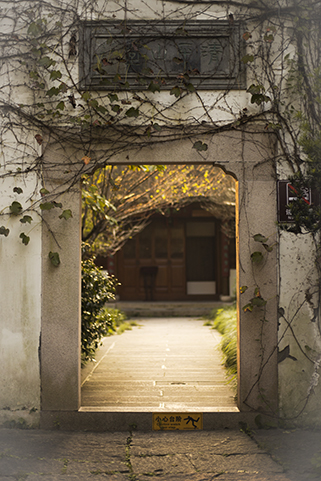
\includegraphics[width=\textwidth]{./Pictures/test.jpg} 
	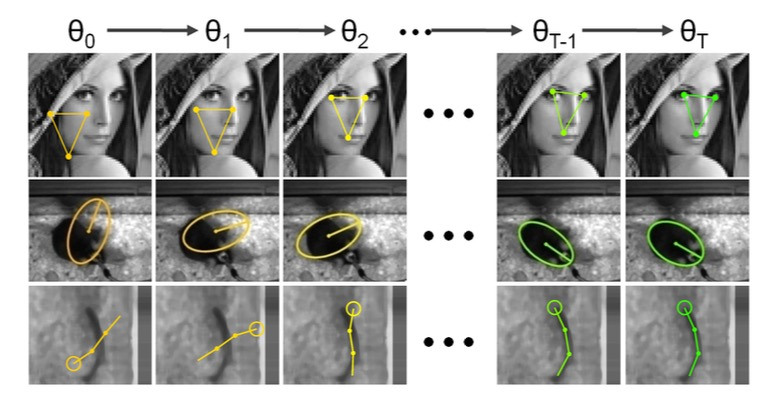
\includegraphics[width=\textwidth]{./mypic/级联回归.jpg} 
	\caption{图像上对物体位姿进行级联回归的一种基本框架} 
\end{figure}

级联回归算法在人脸特征点定位上取得的突破性进展是众多图像回归算法领域最为成功的一个。M. Dantone等人率先利用级联回归框架算法的高效性,并采用条件回归森林作为每一层的回归模型,得到了一种基于模型参数的实时人脸特征点定位算法,并取得了当时最精准的回归精度。同样借鉴于文章[\citenum{dollar2010cascaded}],X. Cao等人在2014年发表了一篇具有突破性意义的人脸特征点定位文章[\citenum{cao2014face}]。这篇文章中提出的人脸特征点回归算法采用非参数化的模型表达,通过直接估计人脸特征点在图像中的坐标位置来实现定位。这种通过直接减少特征点定位精度误差,而不是通过减少模型误差的方式,极大促进了回归精度以及回归速度。能有这样显著的效果提升,极大程度上依赖于级联回归框架的高拟合能力。随后P. Doll{\'a}r再一次总结X. Cao等人的工作经验,利用自己提出的级联回归框架,提出一种能够适应一定人脸被遮挡情况下的人脸特征点定位算法,再一次提高了人脸特征点定位的精准度\cite{burgos2013robust}。在期间也有相关的一些相关的神经网络回归算法被应用到这个领域,但是经过实验证明,神经网络的回归能力和级联回归算法框架下差别不大,但是在计算效率上则远不及级联回归算法\cite{sun2013deep},随后也被慢慢淘汰。最后,R. Shaoqing等人提出了一种里程碑意义的人脸特征点定位算法\cite{ren2014face}。在该算法中,通过提出局部二值特征,并以级联回归学习框架对人脸特征进行学习,从而引导回归模型进行拟合,最后得到了具有极高精度,极高速度并存的人脸特征点定位算法。于此同时,不少类似文章也通过类似的级联回归框架在人脸特征点定位领域取得了相当优秀的成果\cite{cootes2001active}\cite{saragih2009face}\cite{yang2014face}\cite{asthana2014incremental}\cite{kazemi2014one}\cite{burgos2013robust}\cite{xiong2013supervised},具有很高学术借鉴意义。

人脸特征点级联回归回归算法的大致框架如图1-6所示。
首先在训练模型阶段,学习计算出当前特征点处的特征描述,并以此作为下一级回归器的输入,而当前特征点位置与真值之间的偏移量作为下一级回归器的目标回归量。通过大量的真值样本进行训练得到下一级回归模型。此处特征点的位置可以由目标检测器初始化给出,或者是通过上一级的回归模型得到修正之后给出。重复上述过程就可以得到级联回归模型。而在实际测试应用中,通过计算当前特征点位置的特征描述作为当前级拟合回归模型的输入,得到当前目标回归矫正量。将该矫正量叠加到上级特征点位置后可以得到更新后的特征点位置。重复上述过程,完成所有级联回归模型的拟合修正就可以得到最后的人脸特征点位置。这样的模型非常简洁,但具有非常强的拟合能力,能够适应像人脸特征点定位这样具有非常高复杂度回归空间的回归问题,证明了级联回归模型具有相当优秀的实际应用价值。因此本文也希望充分利用这样的级联回归框架,对物体的六维位姿估计问题展开研究。
\begin{figure}[htb]
	\centering 
	% 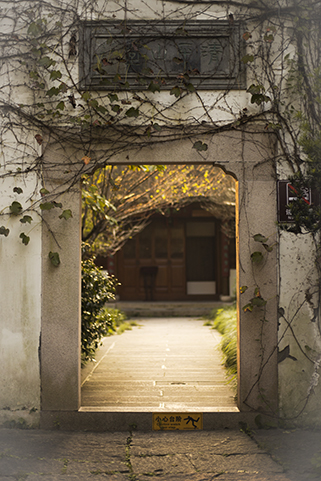
\includegraphics[width=\textwidth]{./Pictures/test.jpg} 
	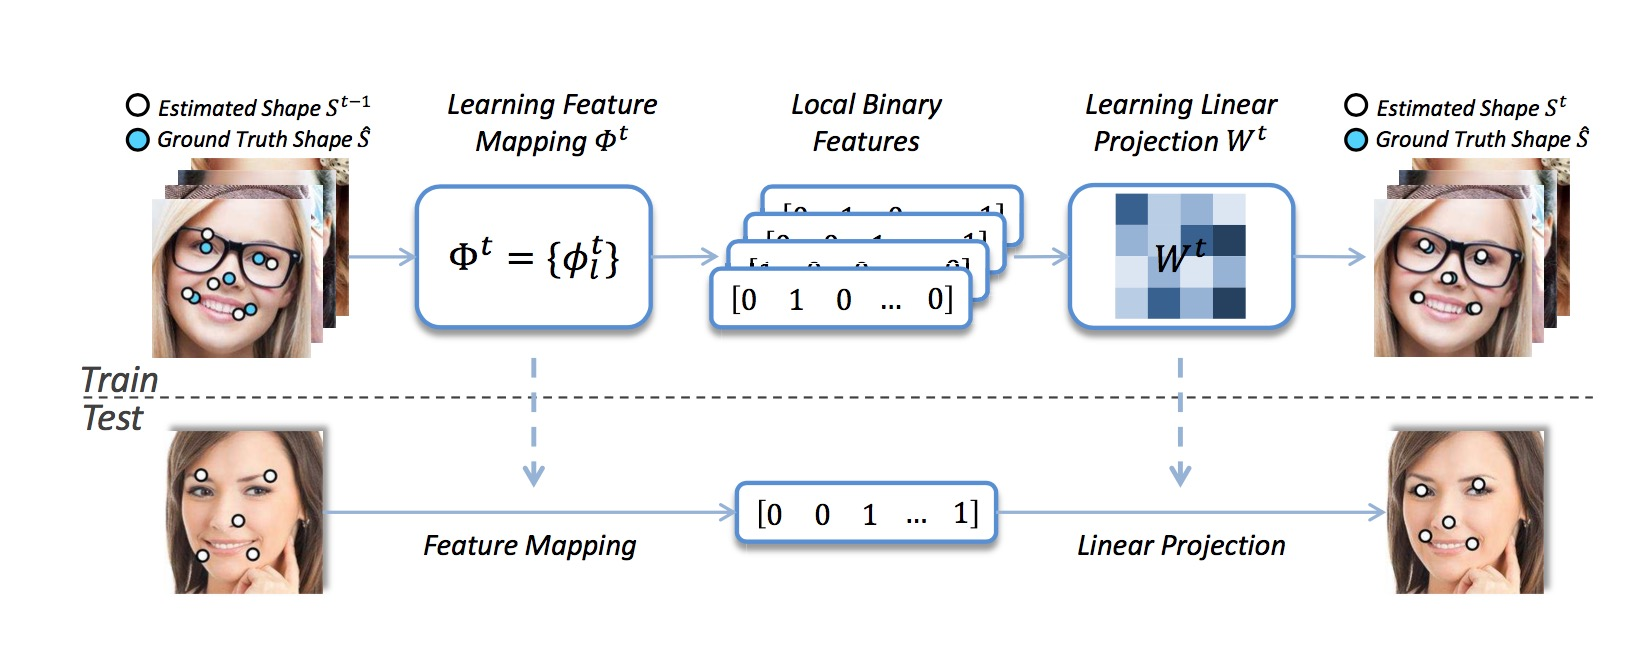
\includegraphics[width=\textwidth]{./mypic/人脸回归算法框架.jpg} 
	\caption{人脸特征点定位问题中的级联回归算法框架} 
\end{figure}

\subsection{物体的六维位姿估计}

物体的六维位姿估计一直以来是机器人领域一个基础问题。早期物体位姿估计的算法研究都是基于工业相机展开的。其中较为成功的几种算法有M. Jones提出的一种基于全局表面特征的位姿估计方法\cite{jones2003fast},以及一些基于局部表面特征的位姿估计方法\cite{schmid1996combining}\cite{rothganger20033d}。随后,D. Thachasongtham等人提出一种更为鲁棒的算法框架,通过事先仿真物体在三维空间中的各个位姿,并通过训练筛选出各个空间位姿下该物体具有的最为稳定的特征点以及相应的特征描述,最后在线测试时通过这些稳定的特征点进行三维位姿匹配\cite{thachasongtham20133d},这样的算法在当时具有一定的大角度变动适应性以及对一些遮挡情况有较好的表现。K. Hara等人研发了一种增长回归随机森林用于对物体的位姿进行直接预测\cite{hara2014growing},但是该增长回归森林算法仅仅可用于分类问题,也就是对物体的直接位姿估计是不够精准的,需要后续其他迭代算法对其结果进行调优。

近些年来,随着深度相机的不断发展,各种新型的深度传感器给机器视觉带来了更丰富的信息来源,深度相机引发了一次物体位姿估计的研究热潮。M. Germann等人搭建了一个3D仿真环境,用于渲染3D模型在空间中的各个位姿,并利用这个仿真提取一些标准深度图像模版,最后通过在线匹配这些深度图像模版与实际深度相机采集到的深度图像进行位姿估计,初步实现了深度图像下的物体六维位姿估计\cite{germann2007automatic}。但由于这个版本的算法需要极大的计算量,文章作者利用GPU进行并行加速计算提高效率,但仍旧无法实现较快的结果输出。随后Park等人改进了其算法,通过简化标准模版之间匹配的过程,同样利用GPU并行处理,提高了该算法框架的实时性,效果得到了显著提升\cite{park2010fast}。图1-7为该类算法一个简易框架示意图,其中最后调优过程一般采用ICP(Iterative Closest Point)算法。
\begin{figure}[htb]
	\centering 
	% 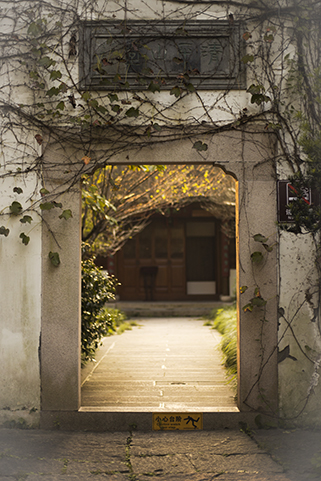
\includegraphics[width=\textwidth]{./Pictures/test.jpg} 
	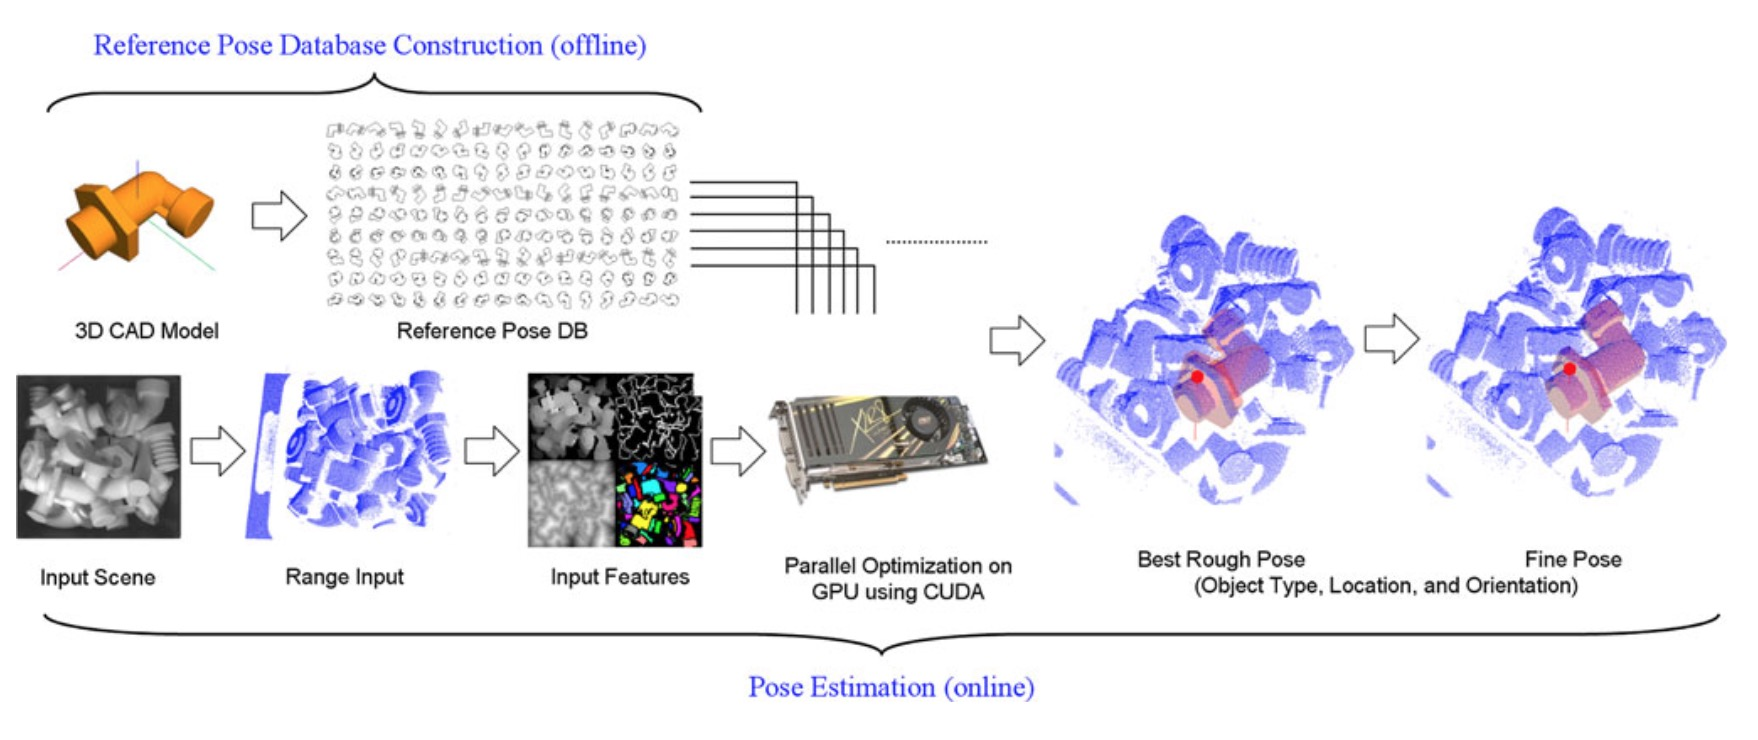
\includegraphics[width=\textwidth]{./mypic/早期位姿估计算法框架.jpg} 
	\caption{早期位姿估计算法框架} 
\end{figure}

为了提高物体位姿估计的实时性,B. Drost等人提出一种基于点云法向量的全局模型特征PPF(Point Pair Features)。这种特征包含了所有模型点云对之间的特性并且与整个模型之间存在一种配对关系,同时具有非常好的计算效率\cite{drost2010model}。利用这种特征描述进行投票机制的位姿估计,使其算法具有非常好的速度以及精度表现。另外S. Hinterstoisser等人则直接利用深度图像计算其对应的梯度响应图作为其特征匹配的基础,得到了非常好的位姿估计效果,同时其计算实时性也非常高\cite{hinterstoisser2012gradient}。他们提出了一种叫做LINE(LINEearizing the memory)特征,包含仅用于深度图像的LINE-2D特征、用于深度图像表面法向量的LINE-3D特征以及用于多模型的LINE-MOD特征。这些特征描述具有非常好的表达能力,是深度图像特征中非常实用的方法。之后他们利用这些特征又提出了一种多模版匹配算法,用于复杂环境下的物体位姿估计,并取得了相当好的效果\cite{hinterstoisser2011multimodal}。

在D. Tang提出潜回归随机森林\cite{tang2014latent}以及J. Gall提出霍夫随机森林\cite{gall2011hough}这两个相当优秀的回归森林算法之后,A. Tejani等人结合这两种算法,提出一种新颖的潜类别霍夫随机森林算法,同时结合LINE-MOD特征用于物体的检测以及六维位姿估计\cite{tejani2014latent}。该算法在当时表现相当出色,取得了State-of-the-art效果。于此同时,E. Brachmann等人采用能量谱图结合随机森林投票的方式也取得了不错的结果,具有较好的借鉴意义\cite{brachmann2014learning}。

随着深度学习的出现和流行,一些基于深度学习的物体位姿框架也逐渐被提出。P. Wohlhart等人提出的一种深度学习特征提取框架能够得到相比LINE-MOD特征更好的特征表述\cite{wohlhart2015learning}。但受限于深度学习框架的庞大性,很难实现高效便捷的算法部署,因此类似的利用深度学习框架进行位姿估计的算法研究成果大都不是特别理想。

得益于人脸特征点定位取得的优秀成果,X. Sun等人将人脸特征点定位算法进行移植改造应用于人手掌的位姿估计中,取得了相当优秀的成果\cite{sun2015cascaded}。该算法通过给手掌指定一些关键点,并设计了一种能适用于深度图像的特征描述方式进行级联回归,能够在不利用GPU并行加速计算的情况下对手掌进行实时位姿估计,同时具备相当准确的位姿回归精度。图1-8为该算法的一个简单流程示意图:
\begin{figure}[htb]
	\centering 
	% 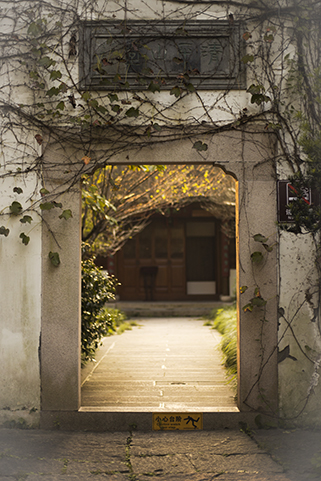
\includegraphics[width=\textwidth]{./Pictures/test.jpg} 
	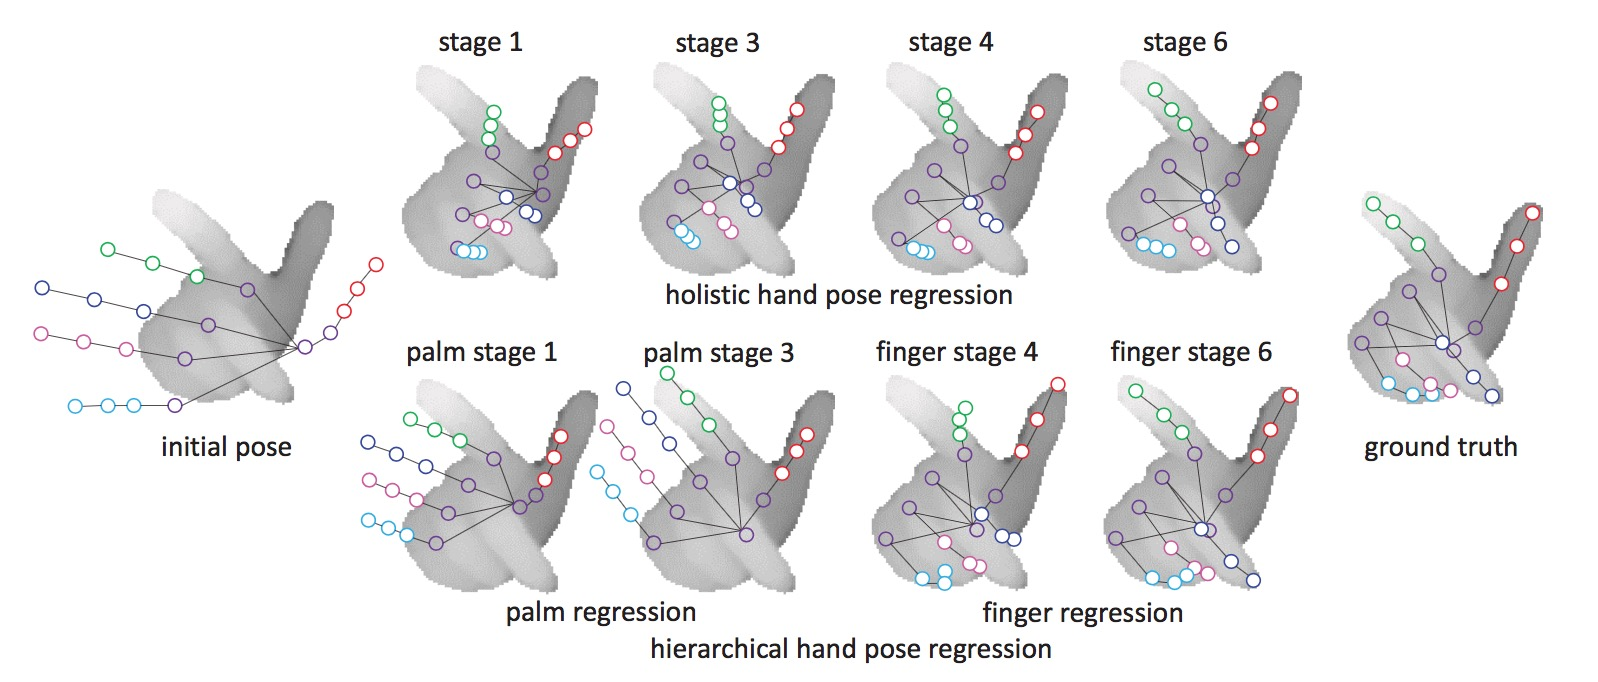
\includegraphics[width=\textwidth]{./mypic/手掌位姿估计流程示意图.jpg} 
	\caption{手掌位姿估计流程示意图} 
\end{figure}
首先在深度图像中给定一个任意的手掌初始位姿,然后通过对关键点的深度图像特征提取,结合随机森林算法进行级联回归最后得到准确的手掌位姿。类似的,E. Brachmann也采用了级联回归框架进行了对通用物体的位姿估计研究,采用RGBD相机作为借口实现了较为理想的位姿估计结果,但在计算效率上略有降低\cite{brachmann2016uncertainty}。这些工作指引物体位姿估计研究的重点放在了级联回归框架上,随后R. Kouskouridas等人进一步改进潜类别霍夫随机森林,实现了物体六维位姿估计高精度情况下的又一次性能提升\cite{kouskouridas2016latent}。

总体而言,物体位姿估计研究在朝着高效率高精度的方向发展。但首先于目前深度相机的精度还并没有非常高,所以目前的研究主要是通过改进算法框架,实现一个更易部署,更为高速的物体位姿估计算法。因此文本也希望能够进一步提高物体位姿估计算法的效率,同时保证其有较好的精度。

\section{本文研究内容}

工业自动化装配流水线背景下,物体的六维位姿估计研究具有如下几个特点:
\begin{itemize}
\item 工业现场需要进行物体位姿估计的场合中,这些物体往往是具有严格尺寸信息的规则刚体,一般都有精确的3D模型。
\item 工业现场很多零件日新月异,每当有一个新的零件需要投入生产时都需要对流水线过程进行更新,或者物体位姿估计算法更新。
\item 工业现场追求效率,所有的应用算法都需要有较高的实时性从而提高生产效率。
\end{itemize}
针对上述这几个现实问题,本文思路为通过继续深入研究随机森林等集成学习算法,进一步提高这类算法的适用性以及鲁棒性,从而使其应用于物体位姿估计领域时能有更好的表现。另一方面为了使物体位姿估计算法具有更好的通用性以及更好的易部署性,本文将考虑利用现有工业条件搭建一个物理仿真环境,方便物体位姿估计算法的快速实现。最后结合级联回归框架得到一个较为完善的工业场景下的物体六维位姿估计方案。

本文最终得到的研究内容可以分为下面这三个大块:
\begin{itemize}
\item 首先以人脸特征点定位这个较为成熟的研究平台来验证随机蕨回归算法的可靠性,以及随机蕨回归算法在面对高维回归空间问题的回归能力和效率。并通过修改经典随机蕨回归框架,通过给算法输入增加一个掩码接口,实现随机蕨回归算法能够有更强的适应性,在针对特征不完备情况下的回归也能合理进行。最后通过实验验证该算法的可行性。
\item 充分利用工业现场可以提供的零件的3D模型信息,借助OpenGL软件平台搭建一个深度相机仿真平台。通过模拟零件在相机视角下的各个位姿,并添加对应的背景以及前景信息,在短时间内生成大量的仿真数据用于后续对物体位姿估计模型的训练。同时,本文将通过修补深度相机产生的空洞以及为仿真深度图像添加随机噪声使其与真实深度图像更为接近,提高仿真程度。
\item 借鉴人脸特征点定位以及文章[\citenum{sun2015cascaded}]中的思路,针对工业现场零件的位姿估计问题设计全新的物体六维位姿级联回归算法框架。并通过设计新的深度图像特征实现物体六维位姿估计算法的高效性。最后利用改进后的随机蕨回归算法,通过对物体的遮挡情况进行估计,实现当物体存在部分被遮挡情况下也能得到较为理想的物体位姿估计结果。
\end{itemize}


\section{本文结构安排}

本文结构安排如下:

第一章主要介绍了在工业环境下本文针对物体位姿估计研究的背景以及意义,并给出了当前集成学习、级联回归算法以及物体六维位姿估计等领域的研究现状。随后给出了本文的主要研究内容以及结构安排。

第二章中先给出了随机蕨算法的经典定义,并通过改造随机蕨算法中的推理公式改造为可以用于回归问题的随机蕨回归算法。然后结合实际应用问题,进一步改造随机蕨算法将其结合特征掩码,介绍如何将随机蕨算法应用到有大噪声干扰的情况中去。最后通过实验验证这些算法改进之后的合理性以及可行性。

第三章主要介绍了在搭建仿真深度相机过程中的数学模型,以及仿真环境搭建的主要流程。其中包括仿真环境中的坐标系设定、旋转关系、OpenGL中的一些基本原理等。并通过进一步为仿真深度图添加人工噪声以及前景背景信息增强其仿真真实度。最后在实验中给出仿真环境的一系列结果。

第四章首先提出了一种可以用于深度图像上的特征提取办法,讨论其尺度不变性,并利用一种监督学习下的特征降维办法对特征进行信噪比提高。然后针对物体的位姿估计提出一种级联回归框架,使其能够实现对通用物体的六维位姿估计。接着进一步讨论物体在存在遮挡情况下如何利用扩展功能后的随机蕨进行针对性处理,以实现复杂环境下的物体位姿估计。最后在本章实验环节中给出了该物体位姿估计算法的可行性以及准确性分析。

第五章给出了本文研究过程中的一些总结,以及对之后的研究工作作出展望。














